\chapter{固体和液体的性质}\label{chapter-properties-of-solids-and-liquids}

\section{晶体和非晶体}
固体可以分成晶体和非晶体两类.在常见的固体中,石英、云母、明矾、食盐、硫酸铜等都是\textbf{晶体},玻璃、蜂蜡、松香、沥青、橡胶等都是\textbf{非晶体}.晶体和非晶体在外形上和物理性质上都有很大区别.

晶体具有天然的规则的几何形状,它的外形是由若干个平面围成的多面体.例如食盐的晶体是立方体(图~\ref{fig_B_4-1a}),明矾的晶体是八面体(图~\ref{fig_B_4-1b}),石英的晶体(透明的石英晶体叫水晶,见图~\ref{fig_B_0-3})中间是六面棱柱,两端是六面棱锥(图~\ref{fig_B_4-1c}).
冬季的雪花是水蒸气在空气中冻结时形成的冰的晶体,它们的形状虽然不同,但都呈六角形的规则图案(见图~\ref{fig_B_0-2}).非晶体则没有规则的外形.

\begin{figure}[htbp]
	\centering
	\begin{subfigure}{0.3\linewidth}
		\centering
		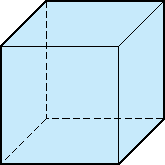
\includegraphics{fig/B/4-1a.pdf}
		\caption{}\label{fig_B_4-1a}
	\end{subfigure}
	\hfil
	\begin{subfigure}{0.3\linewidth}
		\centering
		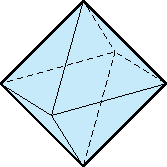
\includegraphics{fig/B/4-1b.pdf}
		\caption{}\label{fig_B_4-1b}
	\end{subfigure}
	\hfil
	\begin{subfigure}{0.3\linewidth}
		\centering
		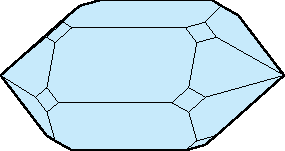
\includegraphics{fig/B/4-1c.pdf}
		\caption{}\label{fig_B_4-1c}
	\end{subfigure}
	\caption{晶体的外形}\label{fig_B_4-1}
\end{figure}


\begin{figure}[htbp]
	\centering
	\begin{minipage}[t]{0.48\linewidth}
		\centering
		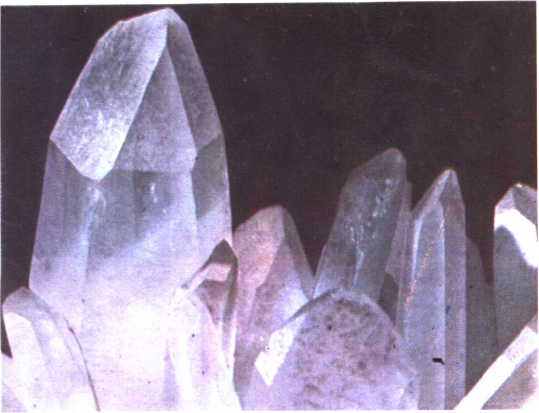
\includegraphics[height=4cm]{fig/B/0-3.png}
		\caption{水晶}\label{fig_B_0-3}
	\end{minipage}
	\begin{minipage}[t]{0.48\linewidth}
		\centering
		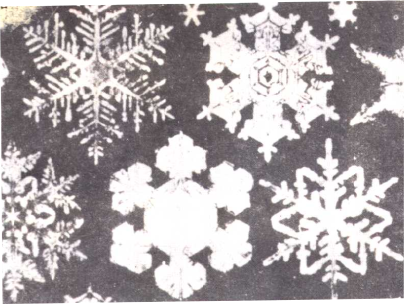
\includegraphics[height=4cm]{fig/B/0-2.png}
		\caption{雪花}\label{fig_B_0-2}
	\end{minipage}
\end{figure}




从实验知道,晶体在不同方向上的物理性质(力学性质、热学性质、电学性质、光学性质等)是不同的.
这种现象叫做晶体的各向异性.以导热性为例,我们来看下面的实验.在一张云母片上涂上很薄一层石蜡,然后用烧热的钢针的针尖
接触云母片,接触点周围的石蜡就熔化了,而熔化了的石蜡成椭圆形(图~\ref{fig_B_4-2}).这表明云母晶体在不同方向上的导热性是不同的.
用玻璃板代替云母片重做上面的实验,熔化了的石蜡则成圆形(图~\ref{fig_B_4-3}),表明非晶体玻璃在不同方向上的导热性是相同的,即各向同性.各向异性是晶体区别于非晶体的一个基本特征,我们可以借助于物体是否具有各向异性来判
断它是不是晶体.

\begin{figure}[htbp]
    \centering
    \begin{minipage}{0.47\linewidth}
    	\centering
    	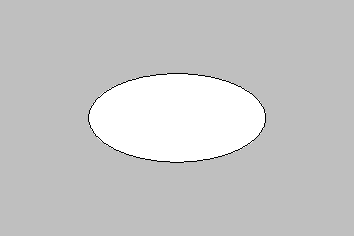
\includegraphics{fig/B/4-2.pdf}
    	\caption{云母片上熔化了的石蜡成椭圆形}\label{fig_B_4-2}
    \end{minipage}
    \hfill
    \begin{minipage}{0.47\linewidth}
    	\centering
    	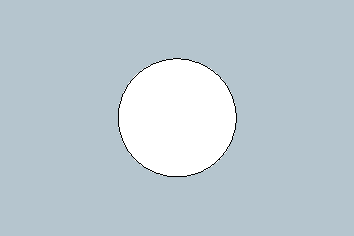
\includegraphics{fig/B/4-3.pdf}
    	\caption{玻璃板上熔化了的石蜡成圆形}\label{fig_B_4-3}
    \end{minipage}
\end{figure}


晶体可以分为单晶体和多晶体.
如果整个物体就是一个晶体,这样的物体就叫做\textbf{单晶体}.
上面说的晶体就是指单晶体.单晶体是科学技术上的重要原材料,制造各种晶体管就要用纯度很高的单晶硅或单晶锗.

如果整个物体是由许多杂乱无章地排列着的小晶体(晶粒)组成的,这样的物体就叫做\textbf{多晶体}.平常见到的\textbf{各种金属材料就是多晶体}.
把纯铁做成的样品放在显微镜下观察,可以
看到它是由许许多多晶粒组成的.晶粒有大有小,最小的只有$10^{-5}$厘米那样大,最大的也超不过$10^{-3}$厘米.每个晶粒都是一个小单晶体,具有各向异性.由于晶粒在多晶体里杂乱无章地排列着,所以多晶体没有规则的几何形状,也不显示各向异性,它在不同方向上的物理性质是相同的,即各向同性.

\section{空间点阵}
十九世纪中叶,人们根据晶体外形的规则性和各向异性提出了一种假说,认为晶体内部的微粒是有规则排列着的.
从1912年开始的应用X射线对晶体结构进行的研究,证实了这种假说的正确.现在,人们用电子显微镜对晶体内部结构进行直接观察和照相,进一步证实了这种假说的正确.

组成晶体的物质微粒(分子、原子或离子)依照一定的规律在空间中排成整齐的行列,构成所谓\textbf{空间点阵}.如果沿着这些物质微粒的行列画出直线来,可以得到若干组平行线,物质微粒就在这些组平行线的交点上.这些交点叫做空间点阵的\textbf{结点}.

晶体中物质微粒的相互作用是很强的,微粒的热运动不足以克服它们的相互作用而远离,因而形成了空间点阵的结构.微粒的热运动主要表现为以结点为平衡位置不停地做微小的振动.


图~\ref{fig_B_4-4} 是食盐的空间点阵示意图.食盐的晶体是由钠离子Na$^+$和氯离子Cl$^-$组成的,它们等距离地交错地排列在三
组相互垂直的平行线上,每个Na$^+$的周围有六个Cl$^-$,每个Cl$^-$的周围有六个Na$^+$.

\begin{figure}[htbp]
	\centering
	\begin{minipage}[t]{0.48\linewidth}
		\centering
		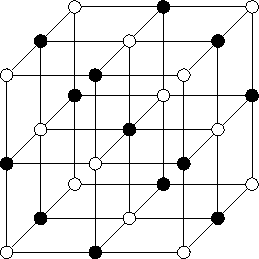
\includegraphics{fig/B/4-4.pdf}
		\caption{食盐晶体的空间点阵}\label{fig_B_4-4}
	\end{minipage}
	\begin{minipage}[t]{0.48\linewidth}
		\centering
		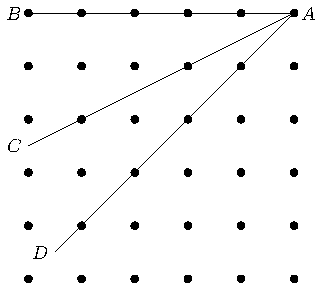
\includegraphics{fig/B/4-5.pdf}
		\caption{各向异性的微观解释}\label{fig_B_4-5}
	\end{minipage}
\end{figure}


晶体外形的规则性可以用物质微粒的规则排列来解释.
同样,晶体的各向异性也是由晶体的内部结构决定的.


图~\ref{fig_B_4-5} 表示在一个平面上晶体物质微粒的排列情况.从图上可以看出,沿不同方向所画的等长直线$AB$、$AC$、$AD$上,物质微粒的数目不同.直线$AB$上物质微粒较多,直线$AD$上较少,直线$AC$上更少.正因为在不同方向上物质微粒的排列情况不同,才引起晶体在不同方向上物理性质的不同.

有的物质能够生成种类不同的几种晶体,是因为它们的物质微粒能够形成不同的空间点阵.例如,碳原子如果按图~\ref{fig_B_4-6} 那样排列就成为石墨,按图~\ref{fig_B_4-7} 那样排列就成为金刚石.石墨是层状结构,层与层之间距离较大,作用力较弱,沿着这个方向容易把石墨一层层地剥下.金刚石中碳原子间的作用力很强,所以金刚石有很大的硬度.
\begin{figure}[htbp]
    \centering
    \begin{minipage}[t]{0.45\textwidth}
        \centering
        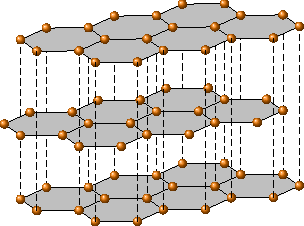
\includegraphics{fig/B/4-6.pdf}
        \caption{石墨的空间点阵}\label{fig_B_4-6}
    \end{minipage}
    \hfil
    \begin{minipage}[t]{0.45\textwidth}
        \centering
        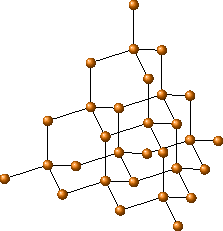
\includegraphics{fig/B/4-7.pdf}
        \caption{金刚石的空间点阵}\label{fig_B_4-7}
    \end{minipage}
\end{figure}


\section{液体的微观结构}
液体的性质介于气体和固体之间.液体一方面像固体,具有一定的体积,不易压缩;另一方面又像气体,没有一定的形状,具有流动性.液体汽化时体积改变上千倍,凝固时体积改变不过百分之十.液体更接近于固体.

跟固体一样,液体中的分子也是密集在一起的,因而液体具有一定的体积,不易压缩.液体分子在很小的区域内作有规则的排列,这种区域是由分子暂时形成的,边界和大小随时改变,有时瓦解,有时又重新形成.液体由大量这种小区域构成,这种小区域杂乱无章地分布着,因而液体表现出各向同性.

液体分子间的距离小,相互作用力还很大,因此液体分子的热运动与固体类似,主要表现为在平衡位置附近做微小的振动.
跟固体不同的是,液体分子没有长期固定的平衡位置,
在一个平衡位置附近振动一小段时间以后,又转到另一个平
衡位置附近去振动,即液体分子可以在液体中移动.
这就是液体具有流动性的原因.

非晶体的微观结构跟液体非常类似,可以看作是粘滞性
极大的液体.所以严格说来只有晶体才能叫做真正的固体.

\section*{阅读材料:液晶}
某些有机化合物(现已发现有几千种)具有一种特殊的物质状态,叫做液晶.液晶一方面像液体,具有流动性;另一方面又像晶体,光学性质具有各向异性.液晶是介于液体和固体之间的过渡状态,微观结构也介于固液之间.

液晶是不稳定的,外界影响的微小变动都会引起液晶分子排列的变化,改变它的光学性质.有一种液晶,在外加电压的影响下,会由透明状态变成混浊状态,不再透明.去掉电压,又恢复透明.
利用这一性质,可以制成显示元件.在两电极间将液晶涂成文字或数码,加上适当电压,透明的液晶变得混浊了,文字或数码就显示出来了.这种显示元件用于电子手表、电子计算器、微电脑以及其他仪器中.

还有一种液晶,具有灵敏的温度效应,温度改变时会改变颜色.只要温度升高1$^\circ$C,液晶就会按红、橙、黄、绿、蓝、靛、紫的顺序改变颜色;温度降低,又按相反顺序改变颜色.液晶的
这种性质,可以用来探测温度.例如在医学上可用来检查肿瘤.在皮肤表面涂上一层液晶,由于肿瘤部分的温度与周围正常组织的温度不一样,液晶会显示出不同的颜色.
电路中的短路点温度高,用同样的办法可检查出短路点.

液晶早在十九世纪八十年代就被发现,直到电子技术和其他一些技术迅速发展起来以后,近十几年来,人们对液晶的研究才有了重要的进展,使它获得了广泛的应用.

\section{液体的表面现象}
荷叶上的小水滴、草叶上的露珠、玻璃板上的小水银滴都是近于球形的.大液滴呈扁平形状,是因为它本身的重量较大,它的形状受到重力的影响也比较大.如果设法消除重力的影响,大液滴也会呈球形.配制水和酒精的混合液,使它的密度跟橄榄油的密度相等.把橄榄油引入这种混合液里,可以看到橄榄油呈球形(图~\ref{fig_B_4-8}).
\begin{figure}[htbp]
    \centering
    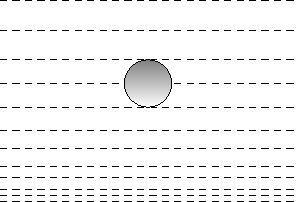
\includegraphics{fig/B/4-8.pdf}
    \caption{橄榄油在水和酒精的混合液里呈球形}\label{fig_B_4-8}
\end{figure}

我们知道,在体积相同的各种形状的物体中,球形物体的表面积最小.
上述实验表明,液体表面有收缩到最小面积的趋势.

我们还可以用肥皂水做实验来证明液面具有收缩趋势.把一根棉线拴在铁丝环上(棉线不要张紧),把环在肥皂水里浸一下,使环上布满肥皂水的薄膜(图~\ref{fig_B_4-9a}).如果用热针刺破棉线左边的薄膜,棉线就被右边的薄膜拉成弧形(图~\ref{fig_B_4-9b});如果刺破右边的薄膜,棉线就被左边的薄膜拉成弧形(图~\ref{fig_B_4-9c}).
\begin{figure}[htbp]
    \centering
    \begin{subfigure}{0.3\linewidth}
        \centering
        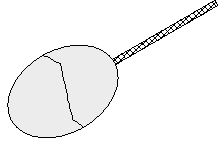
\includegraphics{fig/B/4-9a.pdf}
        \caption{}\label{fig_B_4-9a}
    \end{subfigure}
    \hfil
    \begin{subfigure}{0.3\linewidth}
        \centering
        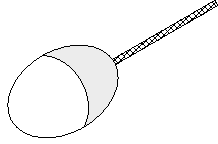
\includegraphics{fig/B/4-9b.pdf}
        \caption{}\label{fig_B_4-9b}
    \end{subfigure}
    \hfil
    \begin{subfigure}{0.3\linewidth}
        \centering
        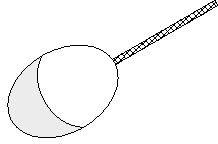
\includegraphics{fig/B/4-9c.pdf}
        \caption{}\label{fig_B_4-9c}
    \end{subfigure}
    \caption{薄膜的收缩使棉线成弧形}\label{fig_B_4-9}
\end{figure}



把一个棉线圈拴在铁丝环上,使环上布满肥皂水的薄膜(图~\ref{fig_B_4-10a}).如果用热针刺破棉线圈里那部分薄膜,外边的薄膜就把棉线圈张紧成圆形(图~\ref{fig_B_4-10b}).


\begin{figure}[htbp]
	\centering
	\begin{subfigure}{0.43\linewidth}
		\centering
		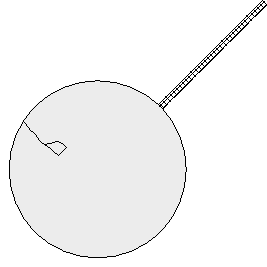
\includegraphics{fig/B/4-10a.pdf}
		\caption{}\label{fig_B_4-10a}
	\end{subfigure}
	\hfil
	\begin{subfigure}{0.43\linewidth}
		\centering
		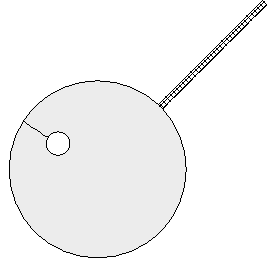
\includegraphics{fig/B/4-10b.pdf}
		\caption{}\label{fig_B_4-10b}
	\end{subfigure}
	\caption{薄膜的收缩使棉线圈成圆形}\label{fig_B_4-10}
\end{figure}


这些实验表明:液体的表面就好像张紧的橡皮膜一样,具有收缩的趋势.

为什么液体表面具有收缩的趋势呢?原来液体跟气体接触的表面形成一个薄层,叫做\textbf{表面层},表面层里的情况跟液体内部有所不同.研究表明,表面层里的分子要比液体内部稀疏些,也就是分子间的距离要比液体内部大些.在液体内部分子间既存在着引力,又存在着斥力.引力和斥力的数量级相同,在通常的条件下可以认为它们的大小是相等的.在表面层里分子间的距离大,引力和斥力都减小,但斥力减小得更快,所以分子间的相互作用表现为引力.
如果在液面上划一条分界线$MN$(图~\ref{fig_B_4-11}),把液面分为(1)和(2)两部分,那么,由于表面层中分子间的引力,液面(1)对液面(2)有引力$f_1$的作用,液面(2)对液面(1)
有引力$f_2$的作用,$f_1$和$f_2$大小相等
方向相反.
像这种液面各部分间相互吸引的力,叫做\textbf{表面张力}.液体的表面张力使液面具有收缩的趋势.
\begin{figure}[htbp]
    \centering
    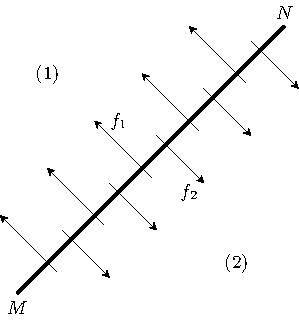
\includegraphics{fig/B/4-11.pdf}
    \caption{液体的表面张力}\label{fig_B_4-11}
\end{figure}

表面张力是跟液面相切的.
如果液面是平面,表面张力
就在这个平面上;如果液面是曲面,表面张力就在这个曲面的切面上.
作用在任何一部分液面上的表面张力,总是跟这部分液面的分界线垂直.

作用在液体表面单位长度分界线上的表面张力,叫做\textbf{表面张力系数}.不同液体的表面张力系数不同.分子间作用力大的液体,表面张力系数大,液态金属的表面张力系数很大,液态气体的很小.

\subsection*{练习一}
\begin{enumerate}
\item 把玻璃管的裂断口放在火焰上烧熔,它的尖端就变圆.这是什么缘故?
\item 在处于失重状态的宇宙飞船中,一大滴水银会呈什么形状?
\item 把熔化的铅一滴一滴地滴入水中,凝固后可以得到
球形的小铅弹.为什么?
\end{enumerate}

\section{浸润和不浸润}
在洁净的玻璃板上放一滴水银,它能够在玻璃板上滚来滚去,而不附着在上面.把一块洁净的玻璃片浸入水银里再取出来,玻璃上也不附着水银.
这种现象叫做\textbf{不浸润}.对玻璃来说,水银是不浸润液体.

在洁净的玻璃板上放一滴水,它要附着在玻璃板上形成薄层.
把一块洁净的玻璃片浸入水里再取出来,玻璃片的表面是带有一层水的.
这种现象叫做\textbf{浸润}.对玻璃来说,水是浸润液体.

同一种液体,对一些固体来说是浸润的,对另一些固体来说是不浸润的.水能浸润玻璃,但不能浸润石蜡.
水银不能浸润玻璃,但能浸润锌.

把浸润液体装在容器里,例如把水装在玻璃容器里,由于水浸润玻璃,器壁附近的液面向上弯曲(图~\ref{fig_B_4-12}).
把不浸润液体装在容器里,例如把水银装在玻璃容器里,由于水银不浸润
玻璃,器壁附近的液面向下弯曲(图~\ref{fig_B_4-13}).
在内径较小的容器里,这种现象更显著,液面形成凹形或凸形的弯月面.

\begin{figure}[htbp]
    \centering
    \begin{minipage}[t]{0.48\textwidth}
        \centering
        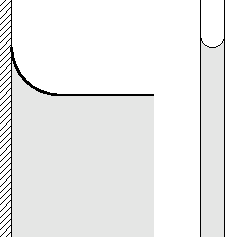
\includegraphics{fig/B/4-12.pdf}
        \caption{液体浸润固体}\label{fig_B_4-12}
    \end{minipage}
    \hfil
    \begin{minipage}[t]{0.48\textwidth}
        \centering
        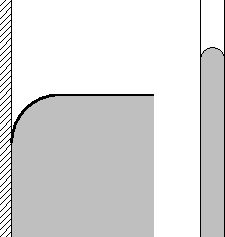
\includegraphics{fig/B/4-13.pdf}
        \caption{液体不浸润固体}\label{fig_B_4-13}
    \end{minipage}
\end{figure}

浸润和不浸润现象也是分子力作用的表现.当液体与固体接触时,在接触处形成一个液体薄层,叫做\textbf{附着层}.附着层里的分子既受到固体分子的吸引,又受到液体内部分子的吸引.如果受到的固体分子的吸引比较弱,附着层里的分子就比液体内部稀疏,在附着层就出现跟表面张力相似的收缩力,这时跟固体接触的液体表面有缩小的趋势,形成不浸润现象.相反,如果受到的固体分子的吸引相当强,附着层里的分子就比液体内部更密,在附着层里就出现液体相互推斥的力,这时跟固体接触的液体表面有扩展的趋势,形成浸润现象.

\subsection*{练习二}

\begin{enumerate}
   \item 把一根缝衣针小心地放在水面上,针可以把水面压弯而不沉没(试试看).解释这个现象.
   \item 布的雨伞虽然纱线间有可以看得出来的孔隙,却仍然不漏雨水.解释这个现象.
\end{enumerate}

\section{毛细现象}
把几根内径不同的细玻璃管插入水中,可以看到管里的水面比容器里的水面高.管的内径越小,管里的水面越高(图~\ref{fig_B_4-14}).如果把这些细玻璃管插入水银中,发生的现象正好相
反,管里的水银面比容器里的水银面低.管的内径越小,管里
的水银面越低(图~\ref{fig_B_4-15}).
\begin{figure}[htbp]
    \centering
    \begin{minipage}[t]{0.48\textwidth}
        \centering
        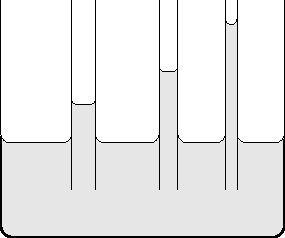
\includegraphics{fig/B/4-14.pdf}
        \caption{浸润液体在毛细管里上升}\label{fig_B_4-14}
    \end{minipage}
    \hfil
    \begin{minipage}[t]{0.48\textwidth}
        \centering
        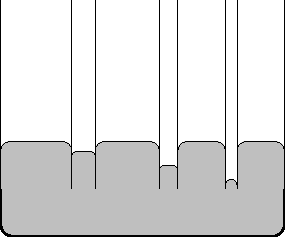
\includegraphics{fig/B/4-15.pdf}
        \caption{不浸润液体在毛细管里下降}\label{fig_B_4-15}
    \end{minipage}
\end{figure}

像这样浸润液体在细管里上升的现象和不浸润液体在细管里下降的现象,叫做\textbf{毛细现象}.发生毛细现象的管叫做毛细管.

浸润液体为什么能在毛细管里上升呢?原来,浸润液体跟毛细管内壁接触时,引起液面的弯曲,使液面变大.而表面张力的收缩作用使液面减小,于是管内液体随着上升,以减小液面.直到表面张力向上的拉引作用和管内升高的液柱的重量达到平衡时,管内液体停止上升,稳定在一定的高度.利用类似的分析,也可以解释不浸润液体在毛细管里下降的现象.

纸张、棉花、毛巾、粉笔、木材、土壤、砖块等物体,内部有
许多细小的孔道,起着毛细管作用,所以它们能够吸水,这就是用毛巾擦汗、灯芯吸油、粉笔吸墨水的道理.

毛细现象在农业生产上有非常重要的意义.
土壤里有很多毛细管,地下的水分可以沿着它们上升到地面.如果要保存地下的水分来供植物的根吸收,就要把地面的土壤锄松,破
坏这些土壤里的毛细管.相反,如果想把地下的水分引上来,就不仅要保持土壤里的毛细管,而且还要使它们变得更细,这时就要用滚子压紧土壤.

\subsection*{练习三}
\begin{enumerate}
\item 要想把凝在衣料上面的蜡或油脂去掉,只要把两层吸墨纸分别放在这部分衣料的上面和下面,然后用熨斗来熨就可以了.
为什么这样做可以去掉衣料上的蜡或油脂?
\item 建筑楼房的时候,在砌砖的地基上铺一层油毡防潮层.如果不铺这层油毡,楼房就容易受潮.为什么?
\end{enumerate}

\section*{复习题}

\begin{enumerate}
\item 晶体和非晶体在外形和物理性质上有什么区别?
\item 什么叫空间点阵?怎样从微观上解释晶体具有规则的外形和各向异性?
\item 液体的微观结构是怎样的?
\item 什么叫表面张力?为什么液体表面具有收缩趋势?
\item 什么叫浸润,什么叫不浸润?怎样解释浸润现象和不浸润现象?
\item 什么叫毛细现象?为什么会发生毛细现象?
\end{enumerate}



